\documentclass[../../main.tex]{subfiles}
    
    \lstset{basicstyle=\small,
      showstringspaces=false,
      commentstyle=\color{black},
      keywordstyle=\color{blue}
    }

    \graphicspath{{../../images/Objekterkennung/}}

    \begin{document}
    \subsection{Objekterkennung}
    Eine zentrale Disziplin um die Anforderungen zu erfüllen ist die Objekterkennung. Um folgende Objekte handelt es sich:

    \begin{itemize}
        \item Würfel
        \item Spur
        \item Signal
    \end{itemize}
    \vspace{0.5cm}

    In diesem Kapitel werden die verschiedenen Lösungskonzepte zur Erkennung dieser Objekte erläutert. Am Ende jedes Kapitels wird zusammenfassend die Bewertung erläutert.

    \textbf{Würfel}\\
    Wie in den Anforderungen beschrieben soll im Startbereich einen Würfel auf den Zug beladen werden. Um die Position des Würfel zu bestimmen muss dieser erkannt werden
    und die Position bestimmt werden. Lösungskonzept "Erkennung mit Ultraschallsensor" und Lösungskonzept "Erkennung mit Stereokamera" werden beschrieben.\\

    \textbf{Spur}\\
    Eine Anforderung an den Schnellzug ist es so schnell wie möglich fahren zu können ohne zu entgleisen. Damit der Zug vor einer Kurve seine Geschwindigkeit
    drosseln kann, muss er die Richtungsänderung der Spur erkennen. Lösungskonzept "Mittels Kamera" und Lösungskonzept "Mittels Sensorwagen" werden beschrieben.\\

    \textbf{Signal}\\
    Das Signal besteht aus einer Tafel, welche am Rand der Gleise aufgestellt werden und auf welcher eine Nummer gedruckt ist. Gemäss Anforderung soll diese Nummer
    während der Fahrt erkennt werden. Ein zweites und kleineres Signal, welches auch am Rand der Gleise aufgestellt wird, soll erkannt werden und so nah wie möglich 
    mit dem Zug an dem Signal anhalten. Lösungskonzept "Mittels Kamera" und Lösungskonzept "Kombination Ultraschallsensor und Kamera" werden beschrieben.


    \subsubsection{Objekterkennung: Würfel}
    Für die Objekterkennung Würfel werden zwei mögliche Lösungskonzepte beschrieben. Die Erkennung mittels Ultraschallsensor und die Erkennung mittels Stereokamera sind zwei mögliche Lösungskonzepte, welche mit unterschiedlichen Disziplinen gelöst werden können(siehe Abbildung \ref{fig:wurfelerkennung}).
    \begin{figure}[H] %Ablaufdiagramm Vision
        \centering
        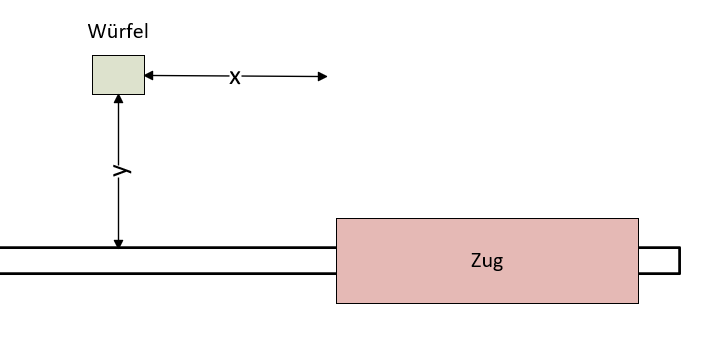
\includegraphics[width=0.5\textwidth]{wurfelerkennung.png}
        \caption{Positionsbestimmung des Würfels}
        \label{fig:wurfelerkennung}
    \end{figure}

    \textbf{Erkennung mittels Ultraschallsensor}\\
    Mittels Ultraschallsensor kann der Würfel erkennt und seine Position ermittelt werden. Der Ultraschallsensor
    wird seitlich am Zug positioniert und misst kontinuierlich den Abstand. Sobald ein Gegenstand mit der Form und
    Grösse des Würfels erkennt wird hält der Zug und der Kran kann sich anhand des ermittelten Abstandes 
    positionieren.
    \begin{figure}[H] %Ablaufdiagramm Vision
        \centering
        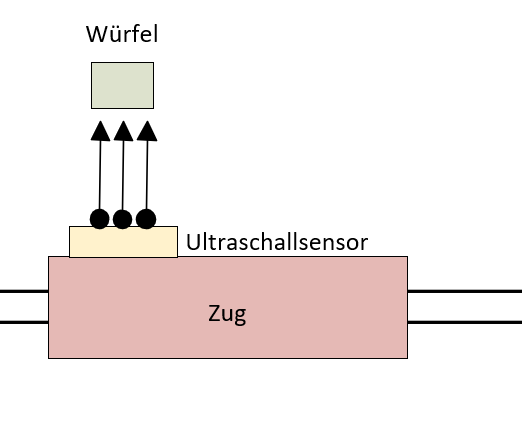
\includegraphics[width=0.4\textwidth]{Ultraschallsensor.png}
        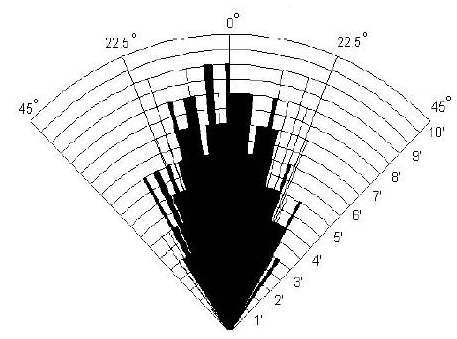
\includegraphics[width=0.4\textwidth]{Ultraschallsensor_angle.png}
        \caption{Objekterkennung und Positionsbestimmung mittel Ultraschallsensor}
        \label{fig:wurfel_ultraschall}
    \end{figure}

    \begin{flushleft}
        \begin{table}[h]
        \begin{tabular}{ | l | p{11cm} |}
        \hline
        \textbf{Problemstellung} & Würfelerkennung \\ \hline
        \textbf{Disziplin} & Elektrotechnik \\ \hline
        \textbf{Lösungskonzept} & Objekterkennung und Positionsbestimmung mittels Ultraschallsensor \\ \hline
        \textbf{Komponente} & Ultraschallsensor HC-SR04 \\ \hline
        \textbf{Bewertung} &  \begin{itemize}
                                \item[+] Schnelligkeit
                                \item[+] Einfachheit
                                \item[+] geringe Kosten 
                                \item[-] weitere Auswertungslogik nötig
                                \item[-] Abstand Zug <=> Würfel limitiert   
                              \end{itemize} \\ \hline
        \end{tabular}
        \caption{Konzeptbeurteilung: Würfelerkennung mittels Ultraschallsensor}
        \label{tab:konzept_wurfel_ultraschall}
    \end{table}
    \end{flushleft}


    \textbf{Erkennung mittels Stereokamera }\\
    Eine weitere Methode den Würfel zu erkennen ist die Objekterkennung mittels Kamera. Hier wird die Kamera am Zug
    befestigt und mittels Software den Würfel gesucht. Um die Position des Würfels im Raum zu ermitteln, wird eine 
    Stereokamera gebraucht. Damit lassen sich Tiefeninformationen und somit den Abstand vom Zug zum Würfel ermitteln.\\
    
    \begin{figure}[H] %Ablaufdiagramm Vision
        \centering
        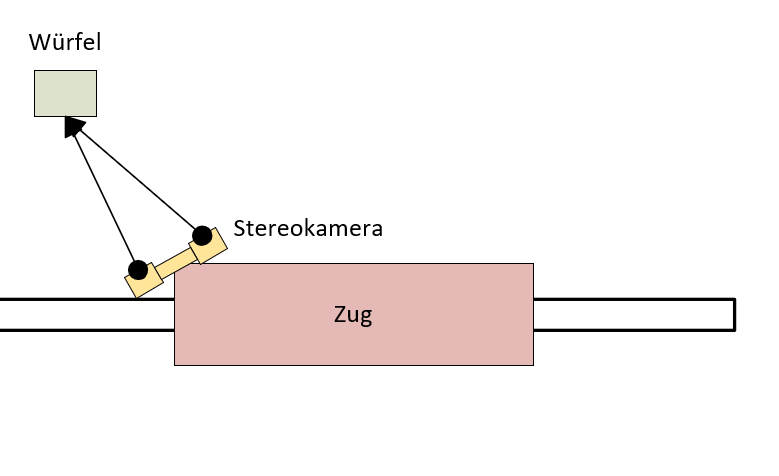
\includegraphics[width=0.4\textwidth]{wurfel_Stereokamera.png}
        \caption{Objekterkennung und Positionsbestimmung mittels Stereokamera}
    \end{figure}

    \begin{flushleft}
        \begin{table}[H]
        \begin{tabular}{ | l | p{11cm} |}
        \hline
        \textbf{Problemstellung} & Würfelerkennung \\ \hline
        \textbf{Disziplin} & Informatik \\ \hline
        \textbf{Lösungskonzept} & Objekterkennung und Positionsbestimmung mittels Stereokamera \\ \hline
        \textbf{Komponente} & Intel RealSense \\ \hline
        \textbf{Bewertung} &  \begin{itemize}
                                \item[+] Hoher Abstandsrange
                                \item[+] Zuverlässigkeit
                                \item[-] hohe Kosten 
                                \item[-] Komplexität
                                \item[-] Schnelligkeit   
                              \end{itemize} \\ \hline
        \end{tabular}
        \caption{Konzeptbeurteilung: Würfelerkennung mittels Stereokamera}
        \label{tab:konzept_wurfel_Stereokamera}
    \end{table}
    \end{flushleft}


    \textbf{Zusammenfassung Objekterkennung Würfel:}\\
    Gemäss der Bewertungen gilt das Lösungskonzept mit dem Ultraschallsensor als die favorisierende Lösung. Als weitere Entscheidungskriterium wurde eine Nutzwertanalyse wie in Abbildung \ref{fig:nutzwer_wurfel} ersichtlich, durchgeführt. Die Lösungsvariante mit dem Ultraschalsensor ist aufgrund seiner Einfachheit und der geringen Kosten die beste Variante.\\ 
    \textbf{Risikoanalyse:}\\
    Die Positionsbestimmung des Würfels ist aufgrund des Variantenentscheids der Mechaniker für den Kran nicht sehr wichtig. Aus diesem Grund sind die Risiken in diesem Bereich klein.\\

    \begin{figure}[H]
        \centering
        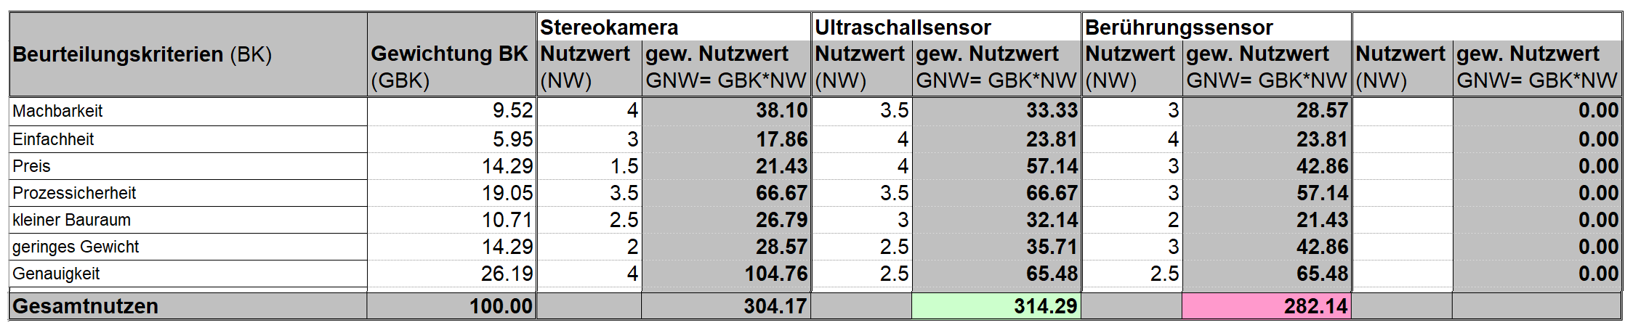
\includegraphics[width=1\textwidth]{Nutzwert_wurfel.png}
        \caption{Nutzwertanalyse Lösungskonzepte Würfel- Erkennung}
        \label{fig:nutzwer_wurfel}
    \end{figure}


    \subsubsection{Spurrichtungserkennung}
	Die «Spurrichtungserkennung» wird gebraucht um so schnell wie möglich mit dem Zug um die Kurven zu fahren. Mit der «Spurrichtungserkennung» muss der Radius der zu fahrenden Kurve so früh wie möglich erkannt werden, damit der Zug auf die richtige Geschwindigkeit gebracht werden kann. Für diese Problemstellung gibt es eine mechatronische- und eine Informatik Lösung.\\

    \textbf{Erkennung mittels Sensorwagen}\\
    Bei der mechatronischen Lösung wird vor dem Zug ein kleiner «Sensor- Wagen» gespannt, welcher mittels einer Achse
    mit dem Zug befestigt ist. Sobald der kleine und leichte «Sensor- Wagen» in die Kurve einfahrt, wird die Achse gedreht
    und somit kann der Radius der Kurve ermittelt werden.\\
    \begin{figure}[H] %Ablaufdiagramm Vision
        \centering
        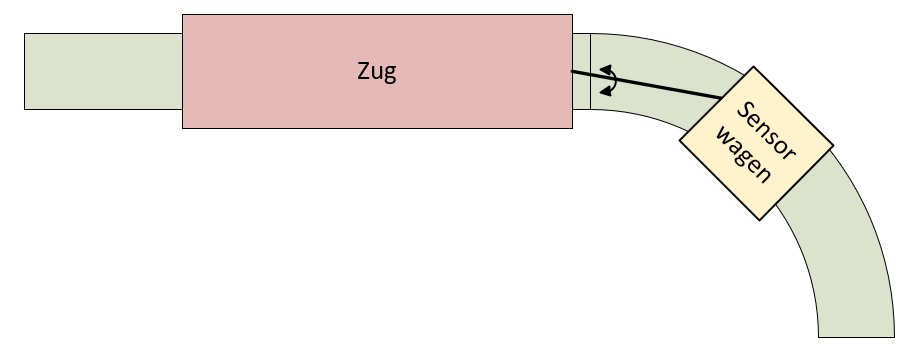
\includegraphics[width=0.6\textwidth]{spurrichtung_mechatronik.png}
        \label{fig:obj_spurrichtung}
        \caption{Spurrichtungserkennung mittels «Sensor- Wagen»}
    \end{figure}

    \begin{flushleft}
        \begin{table}[H]
        \begin{tabular}{ | l | p{11cm} |}
        \hline
        \textbf{Problemstellung} & Spurrichtungserkennung \\ \hline
        \textbf{Disziplin} & Mechatronik \\ \hline
        \textbf{Lösungskonzept} & Erkennung mittels «Sensor- Wagen» \\ \hline
        \textbf{Komponente} & Eigenbau und (Winkelsensor) \\ \hline
        \textbf{Bewertung} &  \begin{itemize}
                                \item[+] Einfachheit
                                \item[+] kostengünstig
                                \item[-] Zuverlässigkeit
                                \item[-] Auflösung   
                              \end{itemize} \\ \hline
        \end{tabular}
        \caption{Konzeptbeurteilung: Würfelerkennung mittels Stereokamera}
        \label{tab:konzept_wurfel_Stereokamera}
    \end{table}
    \end{flushleft}

    \vspace{0.5cm}
    \textbf{Erkennung mittels Kamera}\\
    Eine zweite mögliche Lösung wäre der Einsatz einer Kamera. Die Kamera müsste im unteren Teil des Zuges befestigt
    werden, damit der Spurverlauf gut analysiert werden kann. Wenn die Spur nun die Richtung ändert kann man dies 
    anhand der Kamera feststellen.\\

    \begin{figure}[H] %Ablaufdiagramm Vision
        \centering
        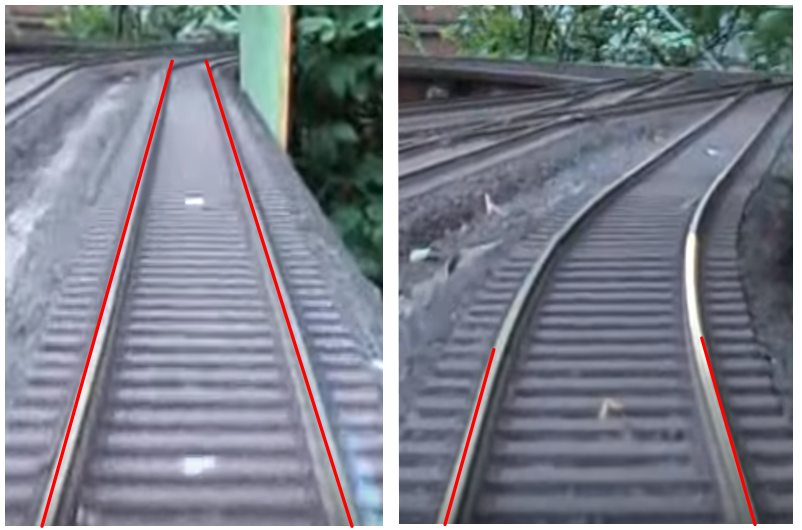
\includegraphics[width=0.8\textwidth]{spurrichtung_Kamera.png}
        \caption{Spurrichtungserkennung mittels Kamera}
    \end{figure}

    \begin{flushleft}
        \begin{table}[H]
        \begin{tabular}{ | l | p{11cm} |}
        \hline
        \textbf{Problemstellung} & Spurrichtungserkennung \\ \hline
        \textbf{Disziplin} & Informatik \\ \hline
        \textbf{Lösungskonzept} & Erkennung mittels Kamera \\ \hline
        \textbf{Komponente} & OV5647 \\ \hline
        \textbf{Bewertung} &  \begin{itemize}
                                \item[+] Einfachheit (Hardware)
                                \item[+] kostengünstig
                                \item[-] Zuverlässigkeit
                                \item[-] Komplexität (Software)   
                              \end{itemize} \\ \hline
        \end{tabular}
        \caption{Konzeptbeurteilung: Würfelerkennung mittels Stereokamera}
        \label{tab:konzept_wurfel_Stereokamera}
    \end{table}
    \end{flushleft}

    \textbf{Zusammenfassung Objekterkennung Spur:}\\
    Bei der Spurerkennung wird auf das Lösungskonzept mit Kamera gesetzt. Die Punkte Einfachheit und Kostengünstig sind die Entscheidungskriterien für den Entscheid. Auch gemäss Nutzwertanalyse \ref{fig:nutzwer_spur} erreicht die Lösung mit Kamera am meisten Punkte.\\
    \textbf{Risikoanalyse:}\\
    Hier besteht ein hohes Risiko im Bereich der Geschwindigkeit. Der Zug soll so schnell wie möglich fahren können. Mit der Kamera und der Spurerkennung und der verwendeten Rechenhardware sind der Geschwindigkeit Limiten gesetzt. Wenn höhere Geschwindigkeiten erreicht werden müssen, muss man auf die alternative Lösung mit Sensorwagen umsteigen.\\

    \begin{figure}[H]
        \centering
        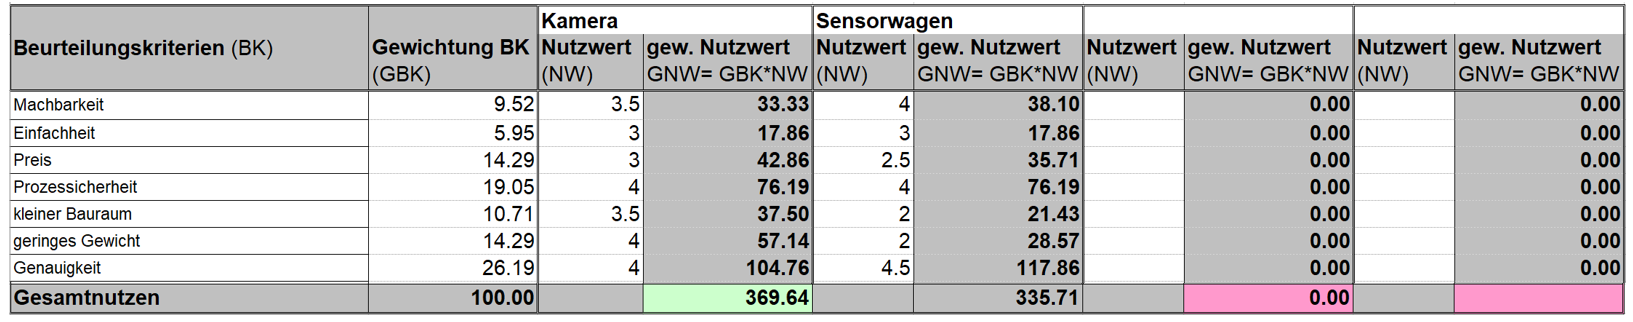
\includegraphics[width=1\textwidth]{Nutzwert_Spur.png}
        \caption{Nutzwertanalyse Lösungskonzepte Spurerkennung}
        \label{fig:nutzwer_spur}
    \end{figure}

    \subsubsection{Signalerkennung}
    Die Signalerkennung besteht aus zwei Teilproblemen. Erstes Teilproblem ist die Erkennung der Tafel, 
    auf welcher die Nummer draufsteht. Die Signaltafel gibt es in zwei Ausführungen - das hohe Signal und das 
    niedrige Signal. Das zweite Teilproblem besteht darin, die auf der Tafel aufgedruckte Zahl zu erkennen.\\

    \begin{figure}[H]
        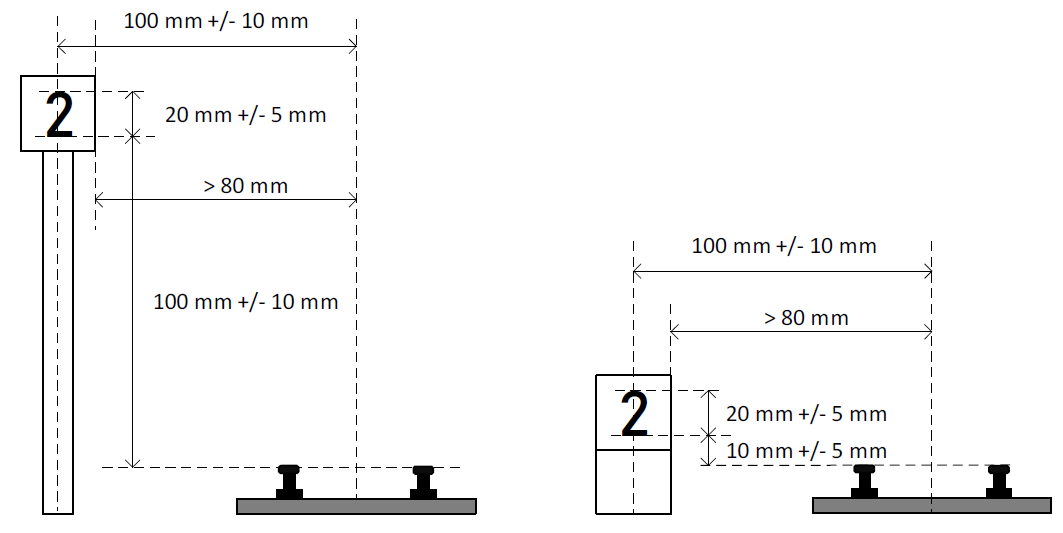
\includegraphics[width=0.8\textwidth]{Signal.png}
        \caption{Auszug aus der Aufgabenstellung: Signaltafel}
    \end{figure}

    Um das Problem «Signalerkennung» zu lösen gibt es eine reine Kamera- Lösung oder eine kombinierte
    Lösung.

    \textbf{Erkennung mittels Kamera:}
    Bei der Informatiklösung setzt man auf eine Objekterkennung mittels Kamera. Die Kamera nimmt während der Fahrt
    kontinuierlich auf und erkennt wenn ein Signal auftaucht. Anschliessend nimmt die Kamera ein Foto der Tafel auf und
    analysiert die aufgedruckte Zahl. 

    \begin{flushleft}
        \begin{table}[H]
        \begin{tabular}{ | l | p{11cm} |}
        \hline
        \textbf{Problemstellung} & Signalerkennung \\ \hline
        \textbf{Disziplin} & Informatik \\ \hline
        \textbf{Lösungskonzept} & Erkennung mittels Kamera \\ \hline
        \textbf{Komponente} & OV5647 \\ \hline
        \textbf{Bewertung} &  \begin{itemize}
                                \item[+] Einfachheit (Hardware)
                                \item[+] kostengünstig
                                \item[-] Schnelligkeit
                                \item[-] Komplexität (Software)   
                              \end{itemize} \\ \hline
        \end{tabular}
        \caption{Konzeptbeurteilung: Signalerkennung mittels Kamera}
        \label{tab:konzept_wurfel_Stereokamera}
    \end{table}
    \end{flushleft}

    \textbf{Erkennung mittels Ultraschallensor und Kamera:}
    Bei der kombinierten Lösung wird das Gesamtproblem in ihre Teilprobleme aufgeteilt und jedes Teilproblem
    individuell gelöst. Zur Erkennung der Tafel wird der Ultraschallsensor verwendet. Dieser an der Seite des Zuges
    angebrachte Sensor detektiert die Tafel und sendet ein Signal zur Kamera. Die Kamera nimmt dann ein Bild von der Tafel
    auf und analysiert die Zahl.\\

    \begin{figure}[H]
        \centering
        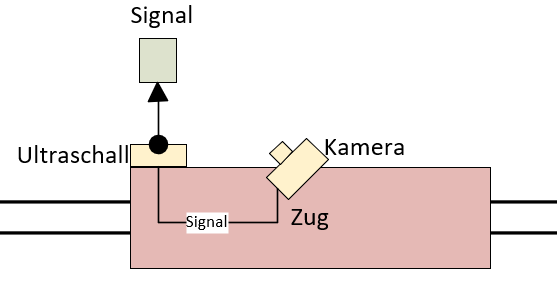
\includegraphics[width=0.7\textwidth]{signal_kombi.png}
        \caption{Signalerkennung mittels Ultraschallsensor und Kamera}
    \end{figure}

    \vspace{1cm}
    \begin{flushleft}
        \begin{table}[H]
        \begin{tabular}{ | l | p{11cm} |}
        \hline
        \textbf{Problemstellung} & Signalerkennung \\ \hline
        \textbf{Disziplin} & Elektrotechnik - Informatik \\ \hline
        \textbf{Lösungskonzept} & Erkennung mittels Ultraschallsensor und Kamera \\ \hline
        \textbf{Komponente} & HC-SR04 / OV5647 \\ \hline
        \textbf{Bewertung} &  \begin{itemize}
                                \item[+] Schnelligkeit
                                \item[+] Einfachheit
                                \item[+] Zuverlässigkeit
                                \item[-] Aufwand (Hardware)   
                                \item[-] Kosten 
                              \end{itemize} \\ \hline
        \end{tabular}
        \caption{Konzeptbeurteilung: Signalerkennung mittels Ultraschallsensor und Kamera}
        \label{tab:konzept_wurfel_Stereokamera}
    \end{table}
    \end{flushleft}

    \textbf{Zusammenfassung Objekterkennung Signal:}
    Bei der Signalerkennung wird auf das Konzept mit der kombinierten Lösung gesetzt. Dies aus dem Grund, dass es schwierig ist eine vernünftige Geschwindigkeit mit dem Zug zu erreichen und gleichzeit eine zuverlässige Signalerkennung mittels Kamera zu gewährleisten. Hier wird bewusst der Mehraufwand für die Hardware in kauf genommen.
    \textbf{Risikoanalyse:}
    Das Risiko wird hier aufgrund der zusätzlichen Absicherung mittels Ultraschallsensor bezüglich Geschwindigkeit minimiert.

    \begin{figure}[H]
        \centering
        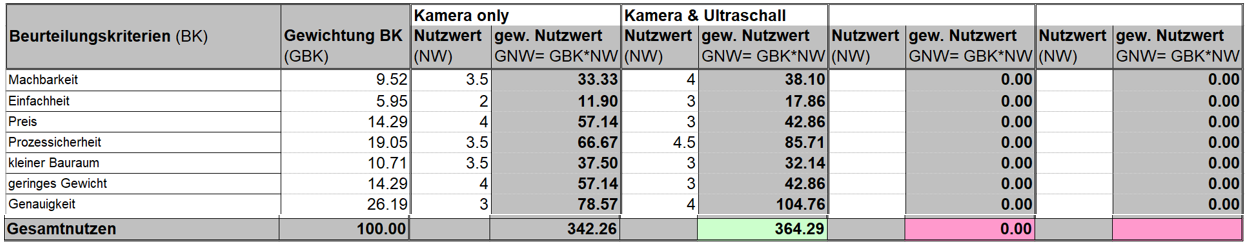
\includegraphics[width=1\textwidth]{Nutzwert_Signal.png}
        \caption{Nutzwertanalyse Lösungskonzepte Signal- Erkennung}
        \label{fig:nutzwer_signal}
    \end{figure}

\end{document}
